\documentclass[11pt]{amsart}
\usepackage[a4paper,margin=1in]{geometry}
\usepackage{amssymb}
\usepackage{booktabs}
\usepackage{tikz}
\usepackage[font=small,labelfont=bf]{caption}
\usepackage[hidelinks]{hyperref}

\colorlet{copper}{orange!75!black}
\colorlet{inkmuted}{black!60}

\newtheorem{theorem}{Theorem}
\newtheorem{proposition}[theorem]{Proposition}
\theoremstyle{remark}
\newtheorem{remark}[theorem]{Remark}

\title{Every Taxicab Distance Once}
\author{Vamshi Jandhyala}
\address{London, United Kingdom}
\email{vamshi.jandhyala@gmail.com}

\begin{document}

\begin{abstract}
Can $n$ points of the integer grid be placed so that their $\binom n2$ taxicab distances are $1,2,\dots,\binom n2$, each exactly once? On a line this asks for a perfect Golomb ruler, which exists only for $n\le4$. A parity count shows that $n$ or $n-2$ must be a perfect square, and placements were known for $n=2,3,4,6,9$. We give a placement of eleven points, the first case beyond those, so a placement exists for every $n\le15$ that the parity count allows. The parity count and the eleven-point placement are formally verified in Lean.
\end{abstract}

\maketitle

\section{The question}

Elliott asked on Mathematics Stack Exchange in September 2024~\cite{MSE}: for which $n$ can $n$ points be placed on the integer grid so that, in the taxicab distance $|x_1-x_2|+|y_1-y_2|$, the $N=\binom n2$ pairs are at distances $1,2,\dots,N$, each exactly once? For $n=3$ the points $(0,0)$, $(0,2)$, $(0,3)$ work, with distances $2$, $3$ and $1$. Before reading on, try $n=4$, and then $n=5$.

On a single line the question asks for a perfect Golomb ruler: marks at which every length from $1$ to the total length is measured exactly once. Equivalently, it asks for a graceful labelling of the complete graph $K_n$, and Golomb showed that one exists only for $n\le4$~\cite{Golomb}. The grid gives the points a second direction, and the answer changes: the asker found placements for $n=6$ and $n=9$ by computer, proved that $n$ or $n-2$ must be a perfect square, and noted that the program was too slow to go further. Its only answer is the author's, giving the placement below.

\begin{theorem}\label{thm:par}
If $n$ points realise every distance $1,\dots,N$ once, and $a$ of them have $x+y$ even and $b$ have $x+y$ odd, then
\[
(a-b)^2=\begin{cases} n, & n\equiv0,1\pmod 4,\\ n-2, & n\equiv2,3\pmod 4.\end{cases}
\]
In particular $n$ is a perfect square when $n\equiv0,1\pmod4$, and $n-2$ is a perfect square otherwise.
\end{theorem}

\begin{proposition}\label{prop:eleven}
The eleven points
\[
\begin{gathered}
\mathrm{A}(0,14),\ \mathrm{B}(0,16),\ \mathrm{C}(1,16),\ \mathrm{D}(7,11),\ \mathrm{E}(8,7),\ \mathrm{F}(11,2),\\
\mathrm{G}(12,7),\ \mathrm{H}(14,45),\ \mathrm{I}(17,49),\ \mathrm{J}(23,0),\ \mathrm{K}(23,26)
\end{gathered}
\]
have taxicab distances $1,2,\dots,55$, each exactly once.
\end{proposition}

The values of $n$ allowed by Theorem~\ref{thm:par} begin $2,3,4,6,9,11,16,18,25,27,\dots$. So a placement exists for $n=2,3,4,6,9,11$ and for no other $n\le15$, and the question is open from $n=16$ on.

\section{The parity count}

Colour each grid point by the parity of $x+y$. A taxicab distance $|x_1-x_2|+|y_1-y_2|$ has the parity of $(x_1+y_1)-(x_2+y_2)$, so it is odd exactly when its endpoints have different colours.

\begin{proof}[Proof of Theorem~\ref{thm:par}]
The pairs of different colours number $ab$, and they realise exactly the odd distances. Among $1,\dots,N$ there are $\lceil N/2\rceil$ odd numbers, so $ab=\lceil N/2\rceil$, and
\[
(a-b)^2=(a+b)^2-4ab=n^2-2N-2\,(N\bmod 2)=n-2\,(N\bmod 2),
\]
using $2N=n^2-n$. Finally $N=n(n-1)/2$ is even exactly when $4$ divides $n(n-1)$, that is, when $n\equiv0$ or $1\pmod4$.
\end{proof}

For $n=5$ the count asks for $(a-b)^2=5$, which is impossible; that is the answer to the warm-up. The proof also fixes the colour classes: their sizes are $\frac12(n\pm\sqrt n)$ or $\frac12(n\pm\sqrt{n-2})$. For $n=11$ that is seven points of one colour and four of the other.

\section{Eleven points}

Figure~\ref{fig:taxi} shows the placement, and Table~\ref{tab:taxi} proves Proposition~\ref{prop:eleven}. Each entry of its upper half is one subtraction in each coordinate and an addition: the distance from H to J, for instance, is $|23-14|+|0-45|=54$. The lower half names, for each $d$ from $1$ to $55$, a pair that the upper half shows is at distance $d$. Fifty-five different distances need fifty-five different pairs, and there are only fifty-five pairs, so each is used once. As Theorem~\ref{thm:par} requires, seven points (C, E, F, G, H, J, K) have $x+y$ odd and four have it even, and $(7-4)^2=11-2$.

\begin{figure}[ht]
\centering
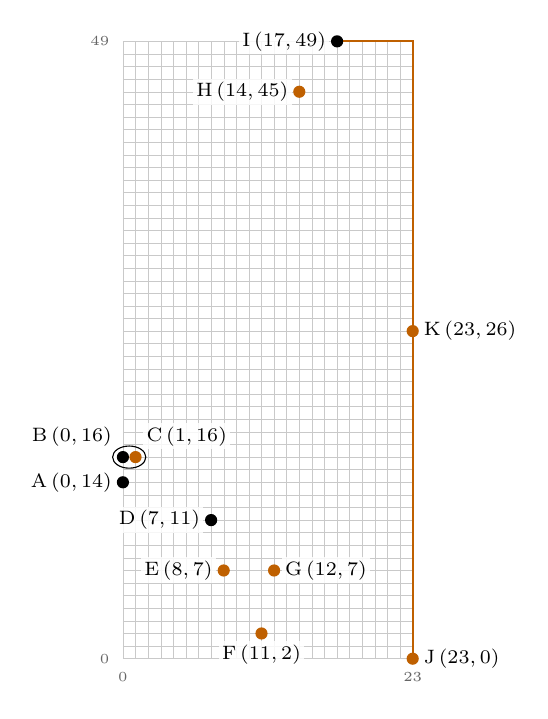
\begin{tikzpicture}
  \draw[line width=0.15pt, inkmuted!35, step=0.16] (0,0) grid (3.680,7.840);
\draw[copper, thick] (2.720,7.840) -- (3.680,7.840) -- (3.680,0.000);
\node[left, font=\scriptsize, inner sep=1.2pt, fill=white, fill opacity=0.85, text opacity=1, outer sep=2.8pt] at (0.000,2.240) {$\mathrm{A}\,(0,14)$};
\node[above left, font=\scriptsize, inner sep=1.2pt, fill=white, fill opacity=0.85, text opacity=1, outer sep=2.8pt] at (0.000,2.560) {$\mathrm{B}\,(0,16)$};
\node[above right, font=\scriptsize, inner sep=1.2pt, fill=white, fill opacity=0.85, text opacity=1, outer sep=2.8pt] at (0.160,2.560) {$\mathrm{C}\,(1,16)$};
\node[left, font=\scriptsize, inner sep=1.2pt, fill=white, fill opacity=0.85, text opacity=1, outer sep=2.8pt] at (1.120,1.760) {$\mathrm{D}\,(7,11)$};
\node[left, font=\scriptsize, inner sep=1.2pt, fill=white, fill opacity=0.85, text opacity=1, outer sep=2.8pt] at (1.280,1.120) {$\mathrm{E}\,(8,7)$};
\node[below, font=\scriptsize, inner sep=1.2pt, fill=white, fill opacity=0.85, text opacity=1, outer sep=2.8pt] at (1.760,0.320) {$\mathrm{F}\,(11,2)$};
\node[right, font=\scriptsize, inner sep=1.2pt, fill=white, fill opacity=0.85, text opacity=1, outer sep=2.8pt] at (1.920,1.120) {$\mathrm{G}\,(12,7)$};
\node[left, font=\scriptsize, inner sep=1.2pt, fill=white, fill opacity=0.85, text opacity=1, outer sep=2.8pt] at (2.240,7.200) {$\mathrm{H}\,(14,45)$};
\node[left, font=\scriptsize, inner sep=1.2pt, fill=white, fill opacity=0.85, text opacity=1, outer sep=2.8pt] at (2.720,7.840) {$\mathrm{I}\,(17,49)$};
\node[right, font=\scriptsize, inner sep=1.2pt, fill=white, fill opacity=0.85, text opacity=1, outer sep=2.8pt] at (3.680,0.000) {$\mathrm{J}\,(23,0)$};
\node[right, font=\scriptsize, inner sep=1.2pt, fill=white, fill opacity=0.85, text opacity=1, outer sep=2.8pt] at (3.680,4.160) {$\mathrm{K}\,(23,26)$};
\fill[black] (0.000,2.240) circle (2.2pt);
\fill[black] (0.000,2.560) circle (2.2pt);
\fill[copper] (0.160,2.560) circle (2.2pt);
\fill[black] (1.120,1.760) circle (2.2pt);
\fill[copper] (1.280,1.120) circle (2.2pt);
\fill[copper] (1.760,0.320) circle (2.2pt);
\fill[copper] (1.920,1.120) circle (2.2pt);
\fill[copper] (2.240,7.200) circle (2.2pt);
\fill[black] (2.720,7.840) circle (2.2pt);
\fill[copper] (3.680,0.000) circle (2.2pt);
\fill[copper] (3.680,4.160) circle (2.2pt);
\draw (0.080,2.560) ellipse (6pt and 4pt);
\node[below, font=\tiny, inkmuted] at (0.000,-0.05) {0};
\node[below, font=\tiny, inkmuted] at (3.680,-0.05) {23};
\node[left, font=\tiny, inkmuted] at (-0.05,0.000) {0};
\node[left, font=\tiny, inkmuted] at (-0.05,7.840) {49};

\end{tikzpicture}
\caption{The eleven points of Proposition~\ref{prop:eleven} in the box $0\le x\le23$, $0\le y\le49$, coloured by the parity of $x+y$: seven copper (odd), four black (even). Every odd distance joins a copper point to a black one. The ringed pair B, C is at distance $1$; the path from I to J, $6$ steps across and $49$ down, has length $55$.}
\label{fig:taxi}
\end{figure}

\begin{table}[ht]
\centering\small
\begin{tabular}{@{}c|rrrrrrrrrr@{}}
 & $\mathrm{A}$ & $\mathrm{B}$ & $\mathrm{C}$ & $\mathrm{D}$ & $\mathrm{E}$ & $\mathrm{F}$ & $\mathrm{G}$ & $\mathrm{H}$ & $\mathrm{I}$ & $\mathrm{J}$\\\hline
$\mathrm{B}$ & 2 &  &  &  &  &  &  &  &  & \\
$\mathrm{C}$ & 3 & 1 &  &  &  &  &  &  &  & \\
$\mathrm{D}$ & 10 & 12 & 11 &  &  &  &  &  &  & \\
$\mathrm{E}$ & 15 & 17 & 16 & 5 &  &  &  &  &  & \\
$\mathrm{F}$ & 23 & 25 & 24 & 13 & 8 &  &  &  &  & \\
$\mathrm{G}$ & 19 & 21 & 20 & 9 & 4 & 6 &  &  &  & \\
$\mathrm{H}$ & 45 & 43 & 42 & 41 & 44 & 46 & 40 &  &  & \\
$\mathrm{I}$ & 52 & 50 & 49 & 48 & 51 & 53 & 47 & 7 &  & \\
$\mathrm{J}$ & 37 & 39 & 38 & 27 & 22 & 14 & 18 & 54 & 55 & \\
$\mathrm{K}$ & 35 & 33 & 32 & 31 & 34 & 36 & 30 & 28 & 29 & 26\\
\end{tabular}\\[1.2em]
\begin{tabular}{@{}rlrlrlrlrl@{}}
1 & BC & 12 & BD & 23 & AF & 34 & EK & 45 & AH\\
2 & AB & 13 & DF & 24 & CF & 35 & AK & 46 & FH\\
3 & AC & 14 & FJ & 25 & BF & 36 & FK & 47 & GI\\
4 & EG & 15 & AE & 26 & JK & 37 & AJ & 48 & DI\\
5 & DE & 16 & CE & 27 & DJ & 38 & CJ & 49 & CI\\
6 & FG & 17 & BE & 28 & HK & 39 & BJ & 50 & BI\\
7 & HI & 18 & GJ & 29 & IK & 40 & GH & 51 & EI\\
8 & EF & 19 & AG & 30 & GK & 41 & DH & 52 & AI\\
9 & DG & 20 & CG & 31 & DK & 42 & CH & 53 & FI\\
10 & AD & 21 & BG & 32 & CK & 43 & BH & 54 & HJ\\
11 & CD & 22 & EJ & 33 & BK & 44 & EH & 55 & IJ\\
\end{tabular}

\caption{Top: the distance between the points labelling each row and column. Bottom: the same $55$ numbers sorted, each with the pair that realises it; reading down the columns runs through $1,\dots,55$.}
\label{tab:taxi}
\end{table}

The smaller placements show how the second dimension helps (Figure~\ref{fig:small}). For $n=3,4$ the points lie on one line, as the Golomb rulers $\{0,2,3\}$ and $\{0,2,5,6\}$. For $n=6$ two adjacent lines suffice. For $n=9$ and $n=11$ the placements found by computer are scattered across the plane.

\begin{figure}[ht]
\centering
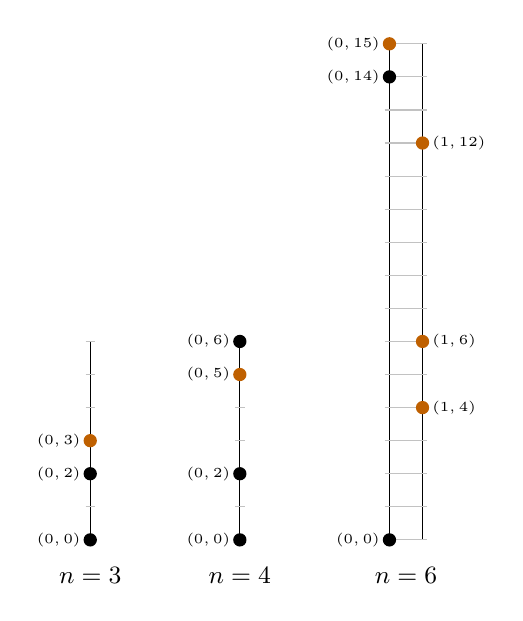
\begin{tikzpicture}
  \draw[thin] (0.000,0) -- (0.000,2.520);
\draw[inkmuted!40] (-0.060,0.000) -- (0.060,0.000);
\draw[inkmuted!40] (-0.060,0.420) -- (0.060,0.420);
\draw[inkmuted!40] (-0.060,0.840) -- (0.060,0.840);
\draw[inkmuted!40] (-0.060,1.260) -- (0.060,1.260);
\draw[inkmuted!40] (-0.060,1.680) -- (0.060,1.680);
\draw[inkmuted!40] (-0.060,2.100) -- (0.060,2.100);
\draw[inkmuted!40] (-0.060,2.520) -- (0.060,2.520);
\fill[black] (0.000,0.000) circle (2.4pt);
\node[left, font=\tiny] at (0.000,0.000) {$(0,0)$};
\fill[black] (0.000,0.840) circle (2.4pt);
\node[left, font=\tiny] at (0.000,0.840) {$(0,2)$};
\fill[copper] (0.000,1.260) circle (2.4pt);
\node[left, font=\tiny] at (0.000,1.260) {$(0,3)$};
\node[font=\small] at (0.000,-0.45) {$n=3$};
\draw[thin] (1.900,0) -- (1.900,2.520);
\draw[inkmuted!40] (1.840,0.000) -- (1.960,0.000);
\draw[inkmuted!40] (1.840,0.420) -- (1.960,0.420);
\draw[inkmuted!40] (1.840,0.840) -- (1.960,0.840);
\draw[inkmuted!40] (1.840,1.260) -- (1.960,1.260);
\draw[inkmuted!40] (1.840,1.680) -- (1.960,1.680);
\draw[inkmuted!40] (1.840,2.100) -- (1.960,2.100);
\draw[inkmuted!40] (1.840,2.520) -- (1.960,2.520);
\fill[black] (1.900,0.000) circle (2.4pt);
\node[left, font=\tiny] at (1.900,0.000) {$(0,0)$};
\fill[black] (1.900,0.840) circle (2.4pt);
\node[left, font=\tiny] at (1.900,0.840) {$(0,2)$};
\fill[copper] (1.900,2.100) circle (2.4pt);
\node[left, font=\tiny] at (1.900,2.100) {$(0,5)$};
\fill[black] (1.900,2.520) circle (2.4pt);
\node[left, font=\tiny] at (1.900,2.520) {$(0,6)$};
\node[font=\small] at (1.900,-0.45) {$n=4$};
\draw[thin] (3.800,0) -- (3.800,6.300);
\draw[thin] (4.220,0) -- (4.220,6.300);
\draw[inkmuted!40] (3.740,0.000) -- (4.280,0.000);
\draw[inkmuted!40] (3.740,0.420) -- (4.280,0.420);
\draw[inkmuted!40] (3.740,0.840) -- (4.280,0.840);
\draw[inkmuted!40] (3.740,1.260) -- (4.280,1.260);
\draw[inkmuted!40] (3.740,1.680) -- (4.280,1.680);
\draw[inkmuted!40] (3.740,2.100) -- (4.280,2.100);
\draw[inkmuted!40] (3.740,2.520) -- (4.280,2.520);
\draw[inkmuted!40] (3.740,2.940) -- (4.280,2.940);
\draw[inkmuted!40] (3.740,3.360) -- (4.280,3.360);
\draw[inkmuted!40] (3.740,3.780) -- (4.280,3.780);
\draw[inkmuted!40] (3.740,4.200) -- (4.280,4.200);
\draw[inkmuted!40] (3.740,4.620) -- (4.280,4.620);
\draw[inkmuted!40] (3.740,5.040) -- (4.280,5.040);
\draw[inkmuted!40] (3.740,5.460) -- (4.280,5.460);
\draw[inkmuted!40] (3.740,5.880) -- (4.280,5.880);
\draw[inkmuted!40] (3.740,6.300) -- (4.280,6.300);
\fill[black] (3.800,0.000) circle (2.4pt);
\node[left, font=\tiny] at (3.800,0.000) {$(0,0)$};
\fill[black] (3.800,5.880) circle (2.4pt);
\node[left, font=\tiny] at (3.800,5.880) {$(0,14)$};
\fill[copper] (3.800,6.300) circle (2.4pt);
\node[left, font=\tiny] at (3.800,6.300) {$(0,15)$};
\fill[copper] (4.220,1.680) circle (2.4pt);
\node[right, font=\tiny] at (4.220,1.680) {$(1,4)$};
\fill[copper] (4.220,2.520) circle (2.4pt);
\node[right, font=\tiny] at (4.220,2.520) {$(1,6)$};
\fill[copper] (4.220,5.040) circle (2.4pt);
\node[right, font=\tiny] at (4.220,5.040) {$(1,12)$};
\node[font=\small] at (4.010,-0.45) {$n=6$};

\end{tikzpicture}
\caption{Placements for $n=3$, $4$ and $6$, coloured by the parity of $x+y$. The first two are Golomb rulers; the six points $(0,0)$, $(0,14)$, $(0,15)$, $(1,4)$, $(1,6)$, $(1,12)$ use a second line, one step away.}
\label{fig:small}
\end{figure}

\section{How the placement was found, and what is open}

An exact search places the distances from the largest down: the largest distance not yet realised must join a new point to a placed one, or two new points, and every branch is tried. It finds the placements for $n\le6$, but its running time grows by a factor of about $35$ with each extra point, so it cannot reach $n=11$. The eleven points came from simulated annealing instead, moving one point at a time and accepting moves that reduce, or occasionally increase, the number of distances in $1,\dots,N$ not yet realised. It finds placements for $n=6$ and $9$ in under a second and for $n=11$ in under half a minute.

For $n=16$, the next value the parity count allows, a run of $100$ seconds found nothing. That reflects a short run and is no evidence that sixteen points are impossible. Whether every $n$ allowed by Theorem~\ref{thm:par} can be realised is open; neither the question nor its comments offers any obstruction beyond parity.

\section{Verification}

Theorem~\ref{thm:par} and Proposition~\ref{prop:eleven}, including the colour split, are proved in Lean~4 with Mathlib~\cite{mathlib}: the statement is that the distances of the pairs $i<j$ form the set $\{1,\dots,N\}$ and are pairwise different, and the eleven-point case is a finite check. A Python script checks the parity rule for $n\le400$ and every placement above, and catches two planted errors (counting $\lfloor N/2\rfloor$ odd numbers, and moving one point). Code and Lean files are at~\cite{repo}.

\section*{Acknowledgments}

The question, the parity condition and the first placements, for $n\le9$, are Elliott's (the placements shown here come from our own searches); the remark on Golomb rulers is a comment by Alex Ravsky, and the link with graceful labellings was noted in a comment by vallev. The search, the analysis and the Lean formalisation were carried out with Claude Opus~5.5 (Anthropic). The author is responsible for the content.

\begin{thebibliography}{9}
\bibitem{MSE} Elliott, \emph{The existence of patterns with unique pairwise distances}, Mathematics Stack Exchange question 4967838 (2024), \url{https://math.stackexchange.com/q/4967838}; the eleven-point placement was posted as answer 5150779 (2026).
\bibitem{Golomb} S.~W.~Golomb, \emph{How to number a graph}, in: Graph Theory and Computing, ed. R.~C.~Read, Academic Press, New York, 1972, 23--37.
\bibitem{mathlib} The mathlib Community, \emph{The Lean mathematical library}, in: Proc. 9th ACM SIGPLAN Int. Conf. on Certified Programs and Proofs (CPP 2020), 367--381.
\bibitem{repo} V.~Jandhyala, code and Lean proofs, \url{https://github.com/jvvk/mathematics/tree/main/every-taxicab-distance-once}.
\end{thebibliography}

\end{document}
